\documentclass{article}
\usepackage[utf8]{inputenc}
\usepackage{graphicx}
\usepackage{mwe}

\title{Sym and Geom portfolio}
\author{Alex Sealy }
\date{April 2021}

\begin{document}

\maketitle


\section{Question 1 -  Challenge 3.3.12}
This question is an attempt to prove that 5 subsets of the vertices of a dodecahedron form distinct cubes.
This can be proven through a nice and succinct argument. The dodecahedron has 30 edges. If we pick one of these edges (the yellow edge in Figure 1), then consider the vertices at the end of four edges that are connected to this first edge (the end of the four blue edges in Figure 1), and then connect these four vertices, we form a square (formed by the four red lines on the diagram). 
\begin{figure}[htbp]
\centerline{\includegraphics[width=
1.5in, height=1.5in]{Cube On Dodecahedron.png}}
\caption{Forming the face of a cube from a dodecahedron edge}
\label{fig1}
\end{figure}

We know that each of these four lines form the edge of a square because each line joins two vertices of a face of the dodecahedron, and as the faces of a dodecahedron are all regular pentagons, the length between any two vertices of a single face are the same as any other. The argument may now proceed by two alternate paths: 1) The square formed in Figure 1 can be connected to the four vertices of the dodecahedron that lie opposite it, forming a cube. This can be repeated for each of the 29 other edges, and as a cube has 6 faces - so it has 6 different generating edges via this method. Therefore there are $30/6 = 5$ different cubes within the dodecahedron generated by this method. 
2) Alternatively, we can consider Figure 2 below, which shows the 5 possible ways that two vertices on the face of a dodecahedron could be connected. This demonstrates that the cube formed by joining the square described earlier to its opposite square face can only be formed in 5 different ways, each joining the vertices of the dodecahedron in one of these ways. Either of these approaches demonstrates that there are 5 different cubes that can be made using some of the vertices of a dodecahedron.

\begin{figure}[htbp]
\centerline{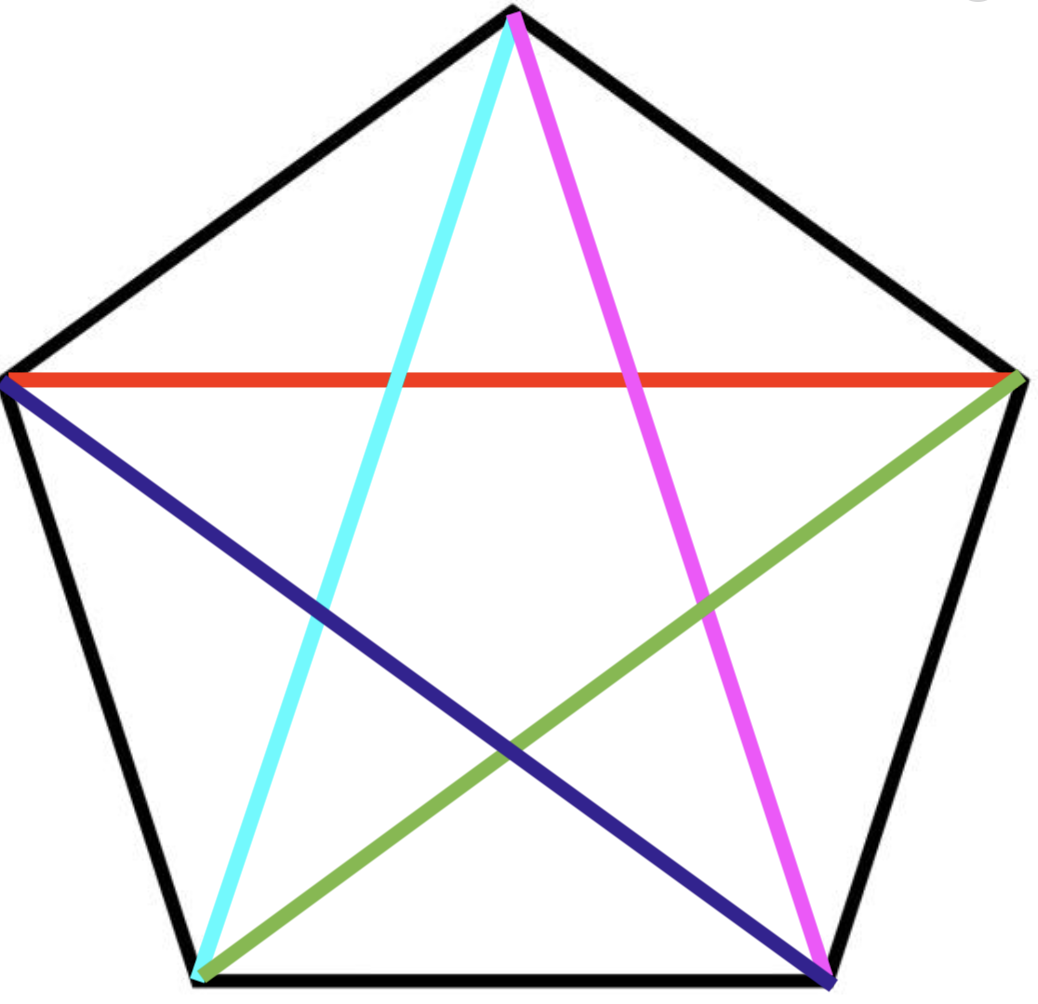
\includegraphics[width=
1in, height=1in]{Pentagon.png}}
\caption{Edge of Cube}
\label{fig2}
\end{figure}

The resulting cube looks like this:
\begin{figure}[htbp]
\centerline{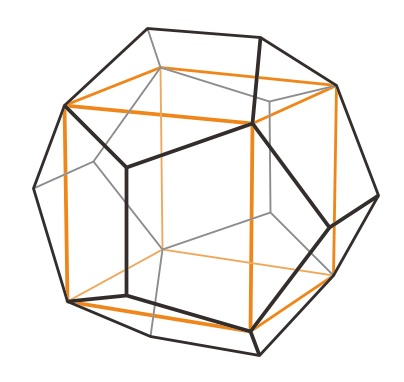
\includegraphics[width=
2in, height=2in]{Cube in Dodo.jpg}}
\caption{Cube in a dodecahedron}
\label{fig3}
\end{figure}



\section{Question 2 - Challenge 4.2.8}
This is an investigation into the Wythoff Construction for $*332$. The Wythoff Construction is useful in identifying both the possible vertex transitive tilings and the possible vertex transitive polyhedra for symmetry groups with signature $*pq2$. $*332$ is a spherical symmetry group and thus, the fundamental domain used in the Wythoff construction must be imagined as a triangle on a sphere. For the sake of ease of diagram, I will portray each construction as a flat triangle. We expect there to be 7 possible Wythoff Constructions for the symmetry group $*332$, which I shall list below:
\begin{figure}[htbp]
\centerline{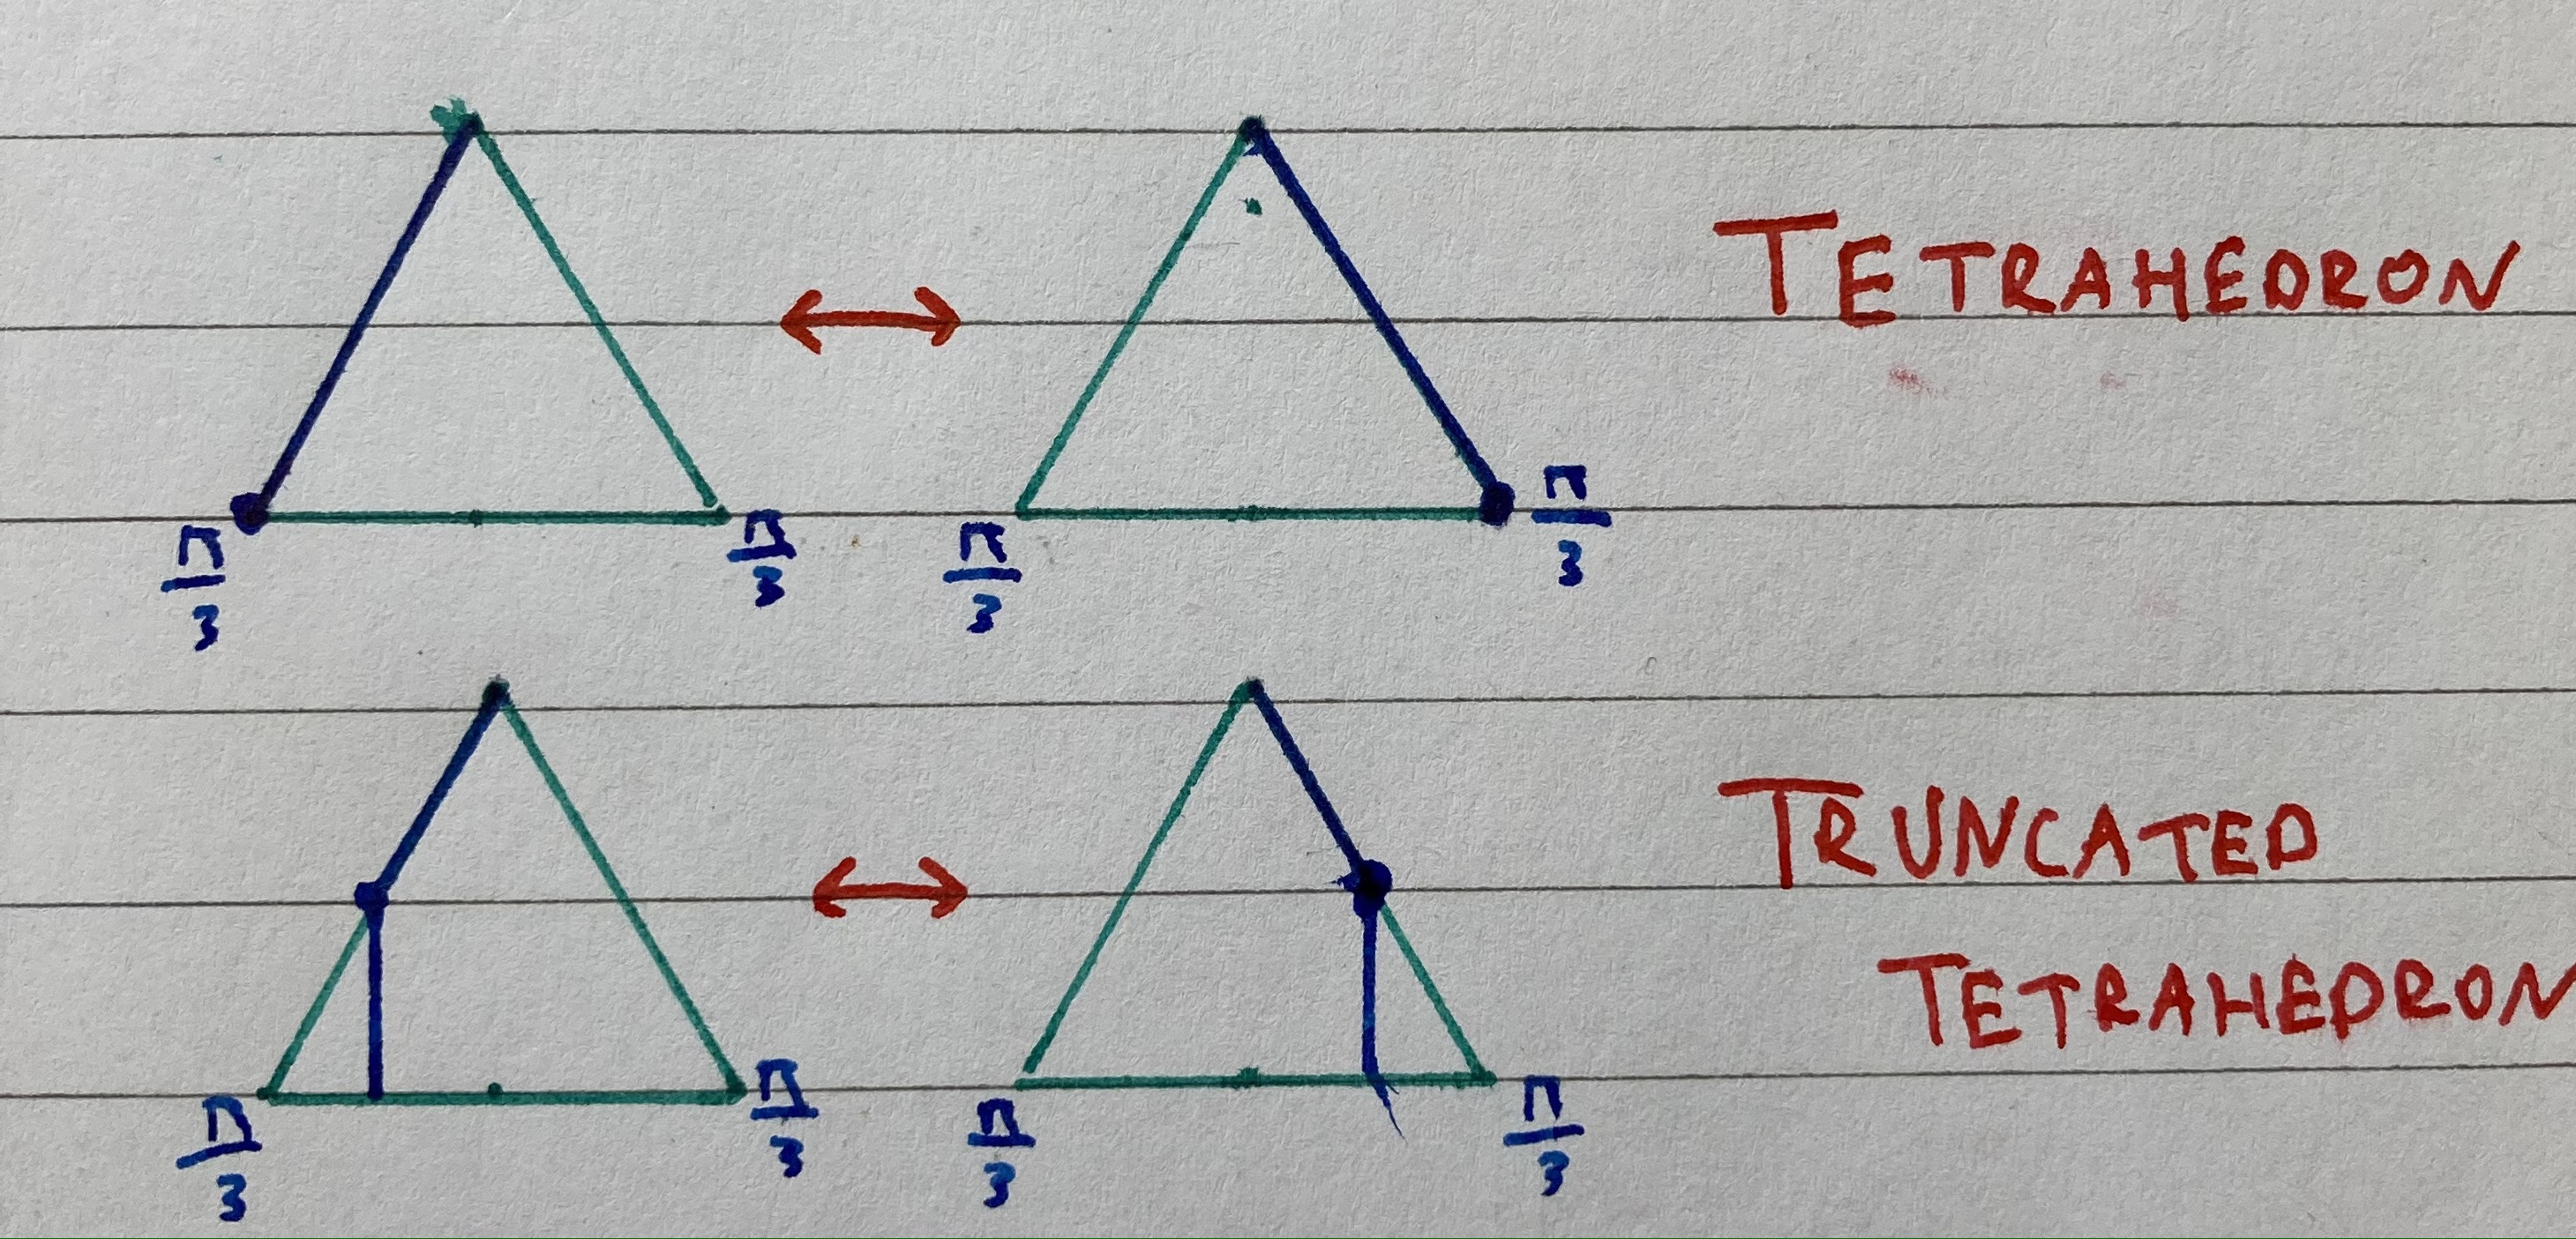
\includegraphics[width=
3in, height=2in]{Wythoff1.JPG}}
\caption{Equivalent Wythoff Diagrams}
\label{fig4}
\end{figure}


Figure 4 displays 4 of the possible 7 Wythoff constructions, however as $p=q$ for the symmetry group $*332$, the triangle used in the Wythoff Diagram is isosceles and thus there are two sets of two equivalent diagrams due to symmetry. These correspond to the Tetrahedron and Truncated Tetrahedron respectively. The former is a Platonic Solid whilst the latter is an Archimedean Solid.

\begin{figure}[htbp]
\centerline{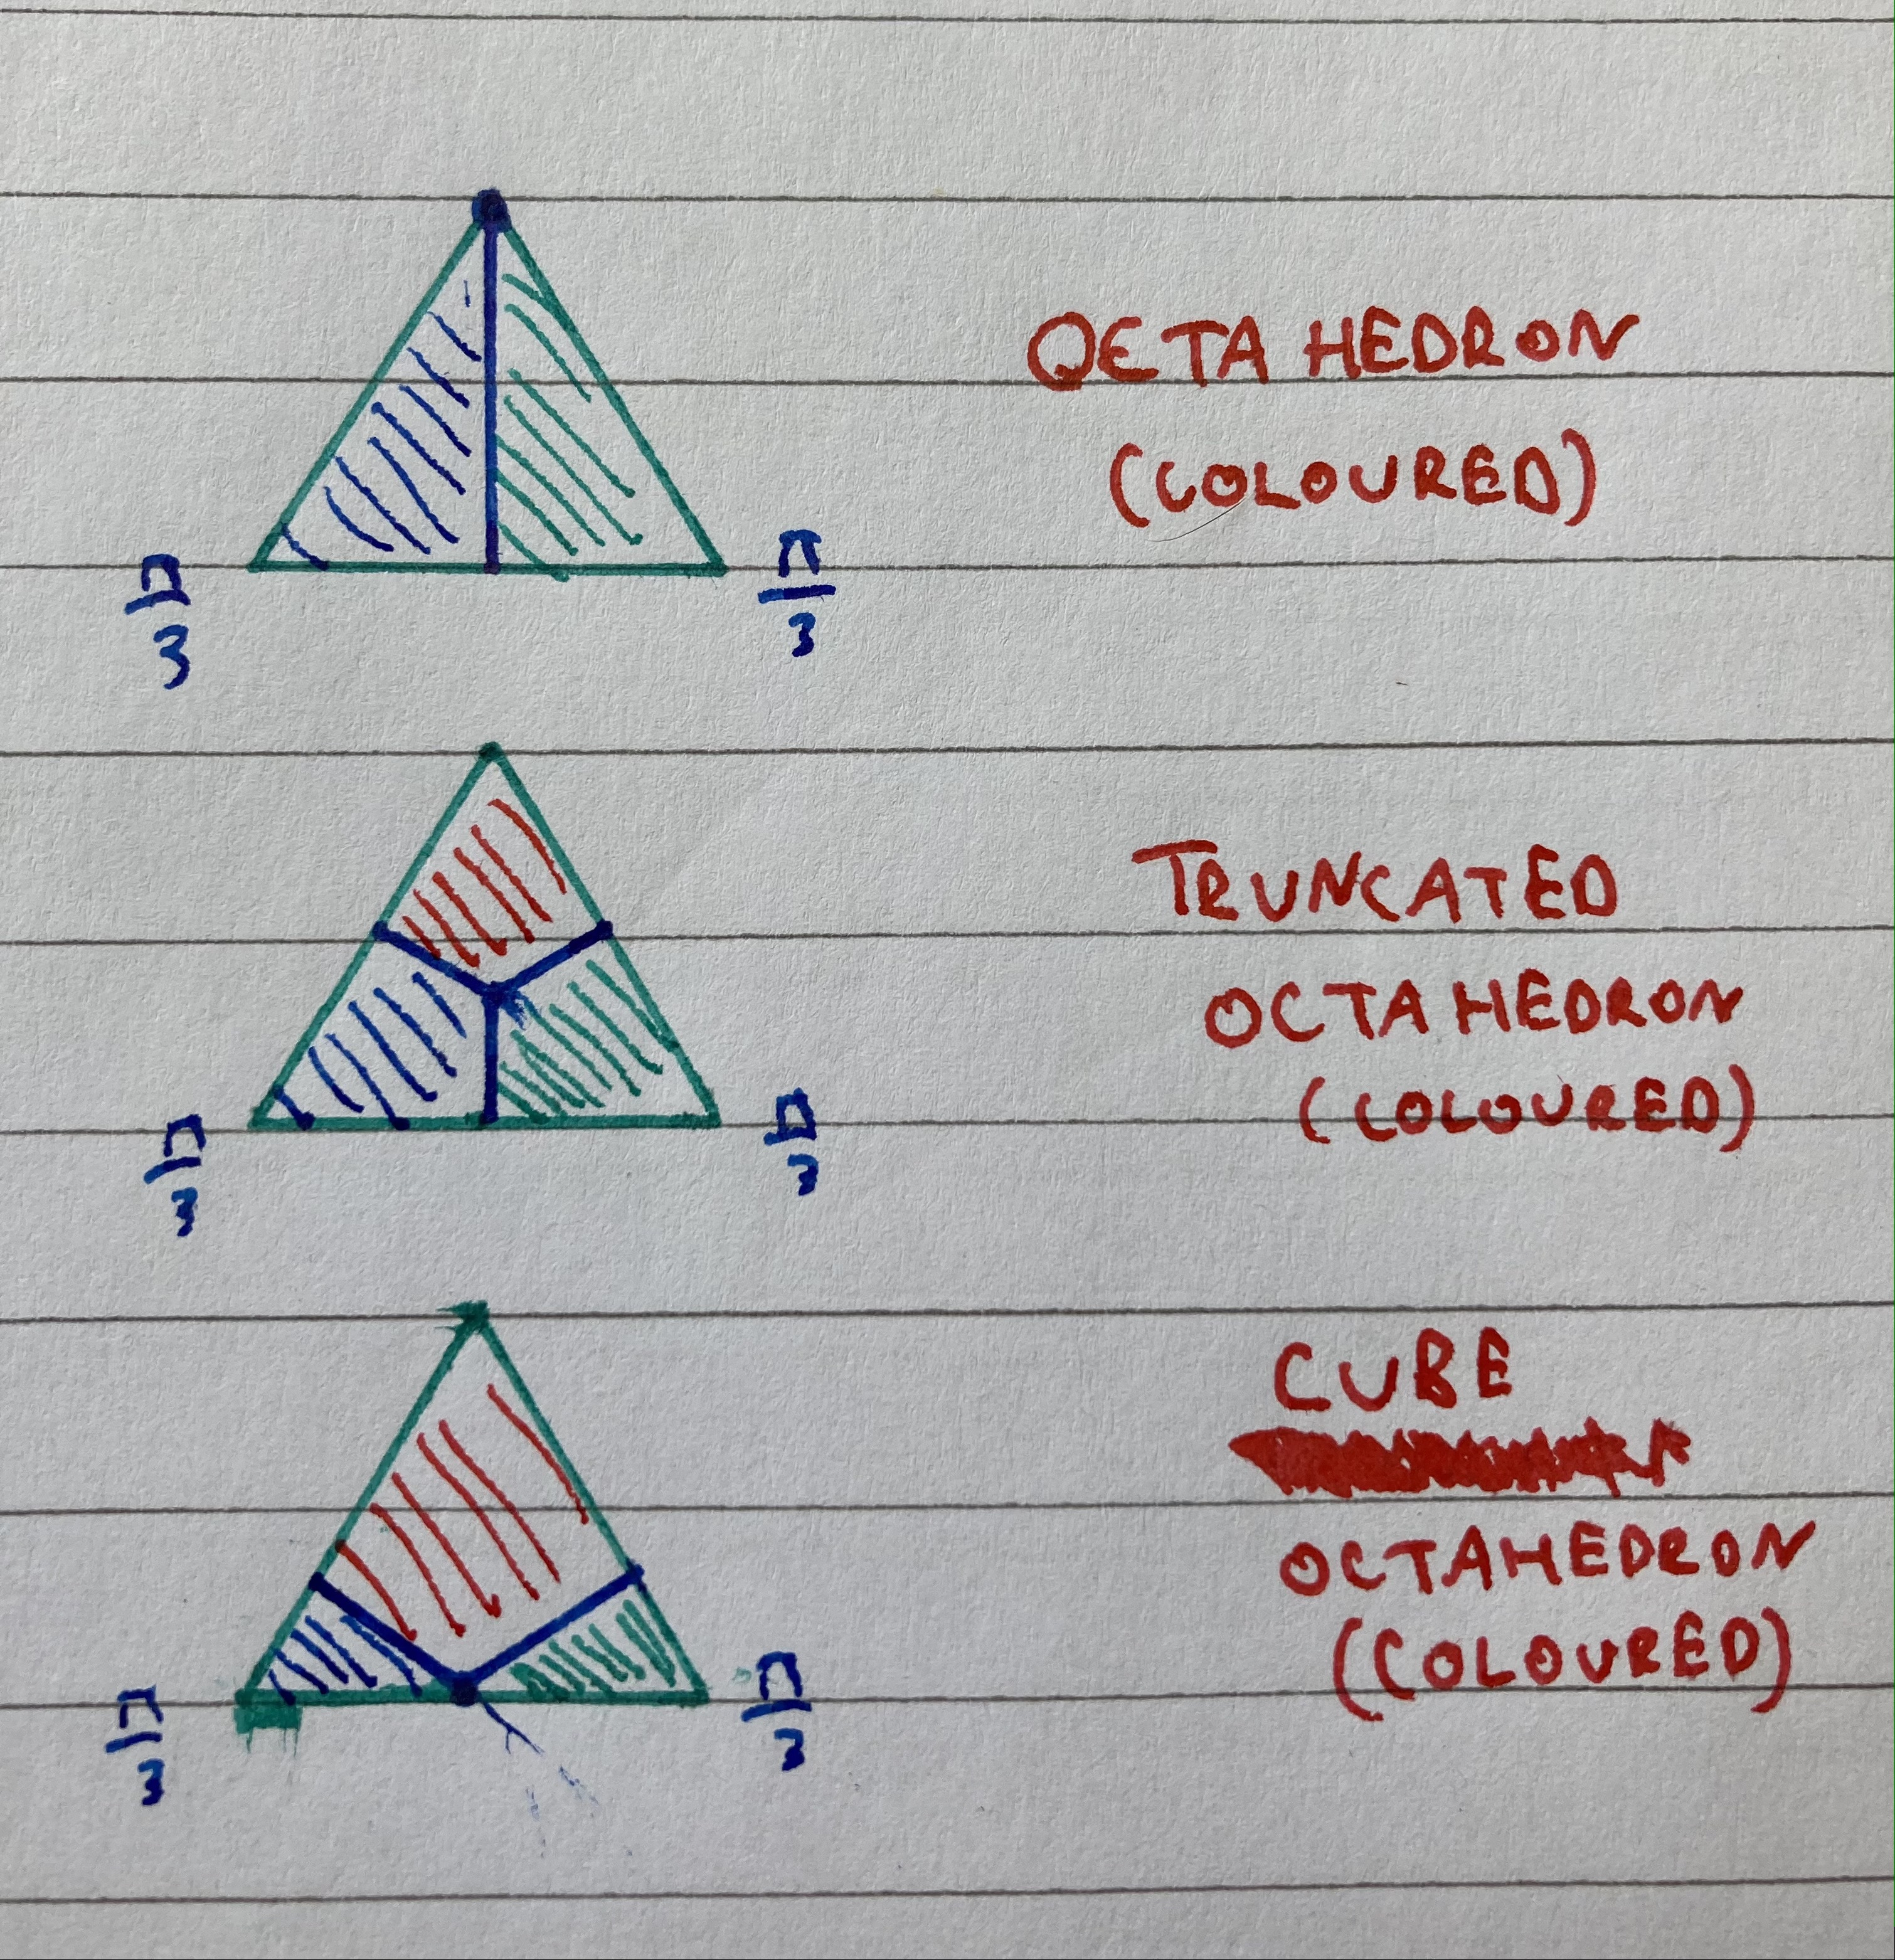
\includegraphics[width=
2.5in, height=3in]{Wythoff2.JPG}}
\caption{Relative Archimedean Wythoff Diagrams}
\label{fig5}
\end{figure}

Figure 5 displays the remaining three possible Wythoff constructions for $*332$, and these correspond to coloured versions of Archimedean and Platonic Solids. The first of these is the regular Octahedron, 2-coloured so that four of its faces are one colour and other four are a different colour and the edges of the faces of one colour never meet the edges of thee faces of another colour. The original octahedron has symmetry group $*432$
\begin{figure}[htbp]
    \centering
    \begin{minipage}{0.3\textwidth}
        \centering
        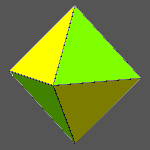
\includegraphics[width=0.9\textwidth]{Coloured Octahedron.png} 
        \caption{2-coloured Octahedron with symmetry group $*332$}
    \end{minipage}\hfill
    \begin{minipage}{0.3\textwidth}
        \centering
        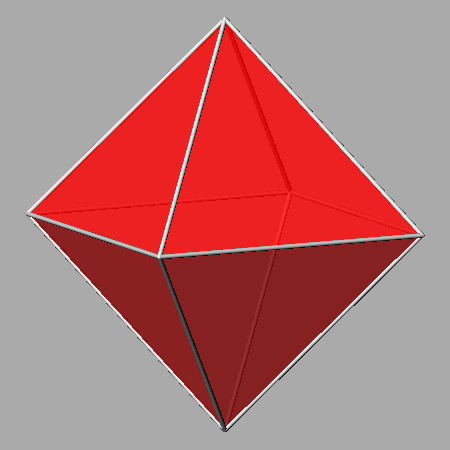
\includegraphics[width=0.9\textwidth]{Octahedron.png} 
        \caption{Normal Octahedron with symmetry group $432$}
    \end{minipage}
\end{figure}

The second of these is the Truncated Octahedron, which despite being having 3 different coloured faces, actually exhibits a 2-colouring, as it is only the hexagonal faces that swap coloring's under any symmetries - the colour of the square faces are fixed.

\begin{figure}[htbp]
    \centering
    \begin{minipage}{0.3\textwidth}
        \centering
        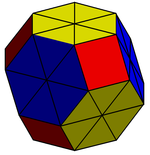
\includegraphics[width=0.9\textwidth]{Truncated Octahedron.png} 
        \caption{2-coloured Truncated Octahedron with symmetry group $*332$}
        
    \end{minipage}\hfill
    \begin{minipage}{0.3\textwidth}
        \centering
        
\includegraphics[width=0.9\textwidth]{Norm Truncated .png} 
        \caption{Normal Truncated Octahedron with symmetry group $*432$}
        
    \end{minipage}
\end{figure}

The third of these is the Cube Octahedron, which again appears to be 3 coloured, but in fact exhibits a 2 colouring as the colour of the square faces remains fixed under any symmetry. The triangular faces are coloured alternatively, so that no vertex of faces of the same colour ever meet.

\begin{figure}[htbp]
    \centering
    \begin{minipage}{0.3\textwidth}
        \centering
        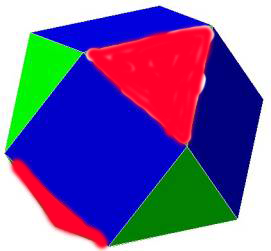
\includegraphics[width=0.9\textwidth]{Cube Octahedron.png}
        \caption{2-coloured Cube Octahedron with symmetry group $*332$}
        
    \end{minipage}\hfill
    \begin{minipage}{0.3\textwidth}
        \centering
        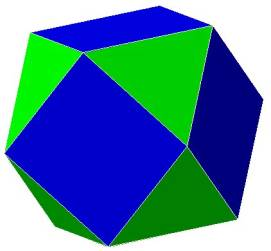
\includegraphics[width=0.9\textwidth]{Normal Cube Octahedron.jpg} 
        \caption{Normal Cube Octahedron with symmetry group $*432$}
       
    \end{minipage}
    
\end{figure}


These last three Wythoff Diagrams of $*332$ result in colored versions of polyhedra that exhibit $*432$ symmetry when they are uncolored. In fact, they are all either Platonic or Archimedean Solids - and their colored subsymmetries are known as "Relative Archimedean Solids" by Conway. 


\section{Question 3 - Challenge 1.5.7}
This is an investigation into the glides that each of the 17 wallpaper patterns might have.
Whilst I will discuss each wallpaper group individually, it is worth noting that whenever a wallpaper group contains a mirror, then it will contain glide symmetries whose glide line lies on that mirror, or parallel to it. So any of the wallpaper groups with mirrors will contain some kind of glide.

I proceed by identifying the point groups($P$) of each wallpaper pattern and using arguments from there to identify what glides each wallpaper pattern has. I have noticed some similarities between certain wallpaper patterns and hence will present them in separate groupings based similarities:

\textbf{First the wallpaper patterns that contain no glides:}

These are the wandering and the purely gyratory wallpaper patterns - those that contain only gyrations. These patterns' point groups are all isomorphic to cyclic groups, as they contain only rotations, and hence do not contain any  lines of reflection to give glide symmetries, and so are devoid of glide symmetries.
\begin{itemize}
  \item $o$ - The wandering is composed solely of translations and thus cannot contain any glide symmetries. It's point group is just the identity - $C_1$

 \item $2222$ - This pattern has four gyratory points of order 2, and thus its point group consists of the identity and a half turn about the origin. Hence $P = C_2$

\item$442$ - This pattern has two distinct gyratory points of order 4 and one of order 2, hence its point group consists of a quarter, half and three quarter turn about the origin, and the identity. Hence $P = C_4$

\item$333$ - This pattern has three distinct gyratory points of order 3, hence its point group consists of a one third and a two third turn about the origin and the identity, hence $P = C_3$

\item$632$ - This pattern has a gyratory point of order 6, 3 and 2, and hence its point group consists of five rotations about the origin and the identity, hence $P = C_6$
\end{itemize}

\textbf{Next are the wallpaper patterns consisting only of mirrors and glides:}

These patterns' point groups are all isomorphic to $D_1$, because they contain only one line of reflection and the identity. 
\begin{itemize}
\item$**$ - This pattern consists of two parallel mirrors. Thus it contains glide symmetries parallel and on top of every mirror line. $P = D_1$
\item$xx$ - This pattern consists solely of miracles, which is a glide achieved without mirror lines. $P = D_1$
\item$*x$ - This pattern consists alternating mirror lines and miracles, thus it contains glides halfway between each mirror line.  $D_1$
\end{itemize}

\textbf{Now I consider the purely kaleidoscopic patterns:}

These patterns all contain glides that reside on top of existing mirror lines and glides halfway between adjacent parallel mirror lines ($*2222$. These latter glides are a result of rotations in the point group being composed with reflections.
\begin{itemize}
\item$*2222$ - The point group consists of two perpendicular reflecting lines, which when composed give a half turn about the origin. Adding the identity forms the point group $P = D_2$ This group does contain any interesting glides because the two mirror lines are perpendicular and the half turn maps between them.
\item$*442$ - The point group consists of four reflecting lines at $45$ degrees to one another, whose composition yields quarter, half and three quarter turns about the origin. Combined with the identity $P = D_4$
\item$*333$ - The point group consists of three mirror lines, who's composition yields a one third and a two third turn around the origin, so with the identity the point group is $P = D_3$
\item$*632$ - The point group consists of six mirror lines, who's composition yields 5 rotations about the origin and with the identity, the point group is $P = D_6$
\end{itemize}
\textbf{Finally the patterns produced by both gyrations and mirrors or glides}:
These patterns have the most interesting glides lines, which are a result of their gyrations in the point group combined with the reflections. In the previous section, the gyrations all lay on the lines of reflection, whereas in this section, the gyrations are independently located. All possess glides on the mirror lines and halfway between adjacent mirror lines, whilst a couple have even more!
\begin{itemize}
\item$22*$ - This pattern contains reflections in one direction only and two order 2 gyrations. The point group so far is the identity, a reflection and a half turn. This does not form a group. The reflection composed with the half turn gives a further glide symmetry which is perpendicular to the original mirror line. Hence $P = D_2$
\item$22x$ - This pattern contains glides in one direction and two order 2 gyrations. The same reasoning as the last pattern can applied to conclude that it also contains glides perpendicular to the original glides. Hence $P = D_2$
\item$2*22$ - This pattern contains reflections in two perpendicular directions, and an order 2 gyration. The point group consists of two perpendicular reflecting lines, the half turn and the identity. Hence $P = D_2$
\item$4*2$ - This pattern contains two perpendicular reflections and an order 4 gyration. The point group consists of reflecting lines, a quarter, two quarter and three quarter turn, the identity, and two distinct glides resulting from the composition of reflections and turns, so $P = D_4$. The glides are thus in between and at $45$ degrees to the original mirror lines.
\item$3*3$ - This pattern contains three mirrors and an order three gyration. The point group is thus three mirrors, two rotations and the identity. Thus $P = D_3$
\end{itemize}

\textbf{In summary} the glides that exist for the 17 wallpaper patterns exist in several forms: on and parallel to existing mirror lines, halfway in between adjacent parallel mirror lines, at $45$ degrees to existing mirror lines, or perpendicular to existing mirror or glide lines.

\end{document}
